\documentclass[conference]{style/acmsiggraph}

\TOGonlineid{45678}
\TOGvolume{0}
\TOGnumber{0}
\TOGarticleDOI{1111111.2222222}
\TOGprojectURL{}
\TOGvideoURL{}
\TOGdataURL{}
\TOGcodeURL{}

\title{Interactive Visualization for System Log Analysis}

\author{Woojong Koh and Armin Samii\thanks{e-mail:\{wjkoh,samii\}@berkeley.edu}\\University of California, Berkeley}
\pdfauthor{Armin Samii and Woojong Koh}

\keywords{visualization, log, data mining, clustering}

\begin{document}

\teaser{
    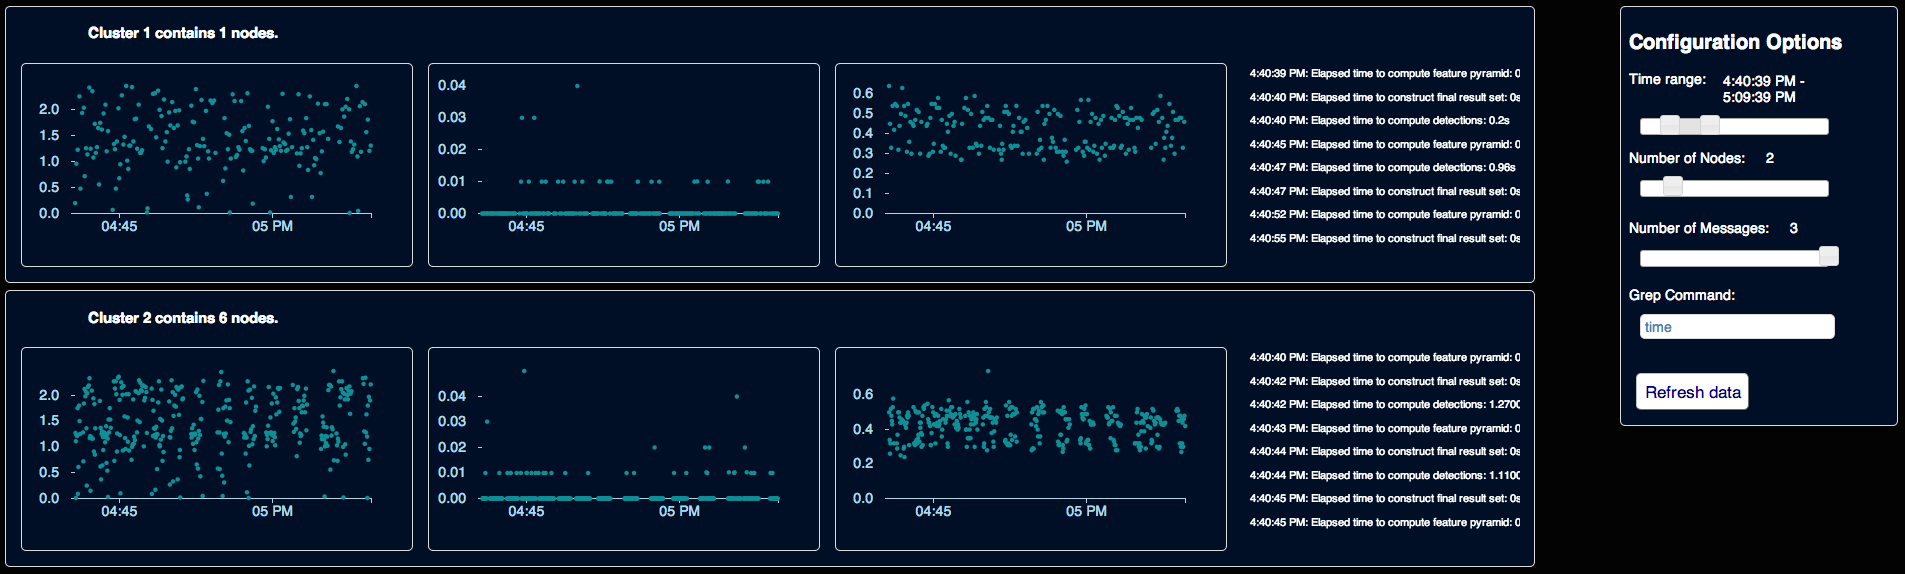
\includegraphics[width=1.0\textwidth]{images/screenshot_full.png}
    \caption{Our visualization displays arbitrary system log data by parsing the variable parts of each log message. Each row contains messages from a single node. Each column is a certain type of message. Each point is a single log message. The x axis is time; the y axis is the value of the extracted variable. The colors indicate multiple variables in the same message. For example, column two has two colors: blue is the number of valid patches, and red is the number of invalid patches. Notice here that five nodes performed similarly (row 2), whereas one node (row 1) is performing more slowly, and thus the number of log messages is sparse. }
}

\maketitle

\begin{abstract}

We present a visualization interface to assist system administrators in searching system logs.
Even with current regular expression matchers such as \texttt{grep}, the amount of log data is difficult for humans to understand.
We augment \texttt{grep} with a visualization of the matched patterns.
To further reduce the amount of information displayed, we cluster similarly-performing nodes and only show a single node representative of the entire cluster.
The user can then interactively search the log, zoom in on a certain time window, and choose the number of clusters.
%This means that at the most ``zoomed out'' state (no time window specified, no search patters, and no clustering), the raw log data is displayed.
Our simulations show that our clustering is effective and our system is fast:
the clustering successfully isolates anomalously-performing nodes in a variety of situations;
the visualization can interactively visualize hundreds of millions of log messages across a hundred nodes in real-time.
TODO: Get the numbers from this simulation.

\end{abstract}

\begin{CRcatlist}
  \CRcat{I.3.3}{Computer Graphics}{Three-Dimensional Graphics and Realism}{Display Algorithms}
  %CRcat{I.3.7}{Computer Graphics}{Three-Dimensional Graphics and Realism}{Radiosity};
\end{CRcatlist}

\keywordlist

%% Use this only if you're preparing a technical paper to be published in the 
%% ACM 'Transactions on Graphics' journal.

\TOGlinkslist

%% Required for all content. 

\copyrightspace

\section{Introduction}

The gears of a distributed system are complex and constantly moving.
A system administrator uses log files to understand the underlying structure and detect anomalous behavior.
These logs are large, distributed across many filesystems, and hard to understand even with today's tools.

Our goal is to aggregate the log data into a visualization that can be easily understood by the system administrator.
The two primary use cases are:
\begin{enumerate}
\item searching through system logs to find software bugs or hardware failures, and
\item viewing the current system state on-the-go without access to a command line.
\end{enumerate}
To this end, our system contributes the following features:
\begin{enumerate}
\item \textbf{trustable}: the user is able to view the raw data at the most ``zoomed out'' state;
\item \textbf{fast and distributed}: the proprocessing primarily occurs at each node, with a single central node aggregating preprocessed data; and
\item \textbf{interactive}: the user can adjust the paramaters of the visualization at interactive speeds.
\end{enumerate}

With a large enough cluster, this will require focusing the user’s attention on “interesting” parts
of the system state. This will require detecting anomalies, which in turn requires a
constantly-evolving model of what the “normal” state of the system is.


\section{Related Work}
% A description of previous papers related to your project.

\begin{figure*}[p]
    \centering
    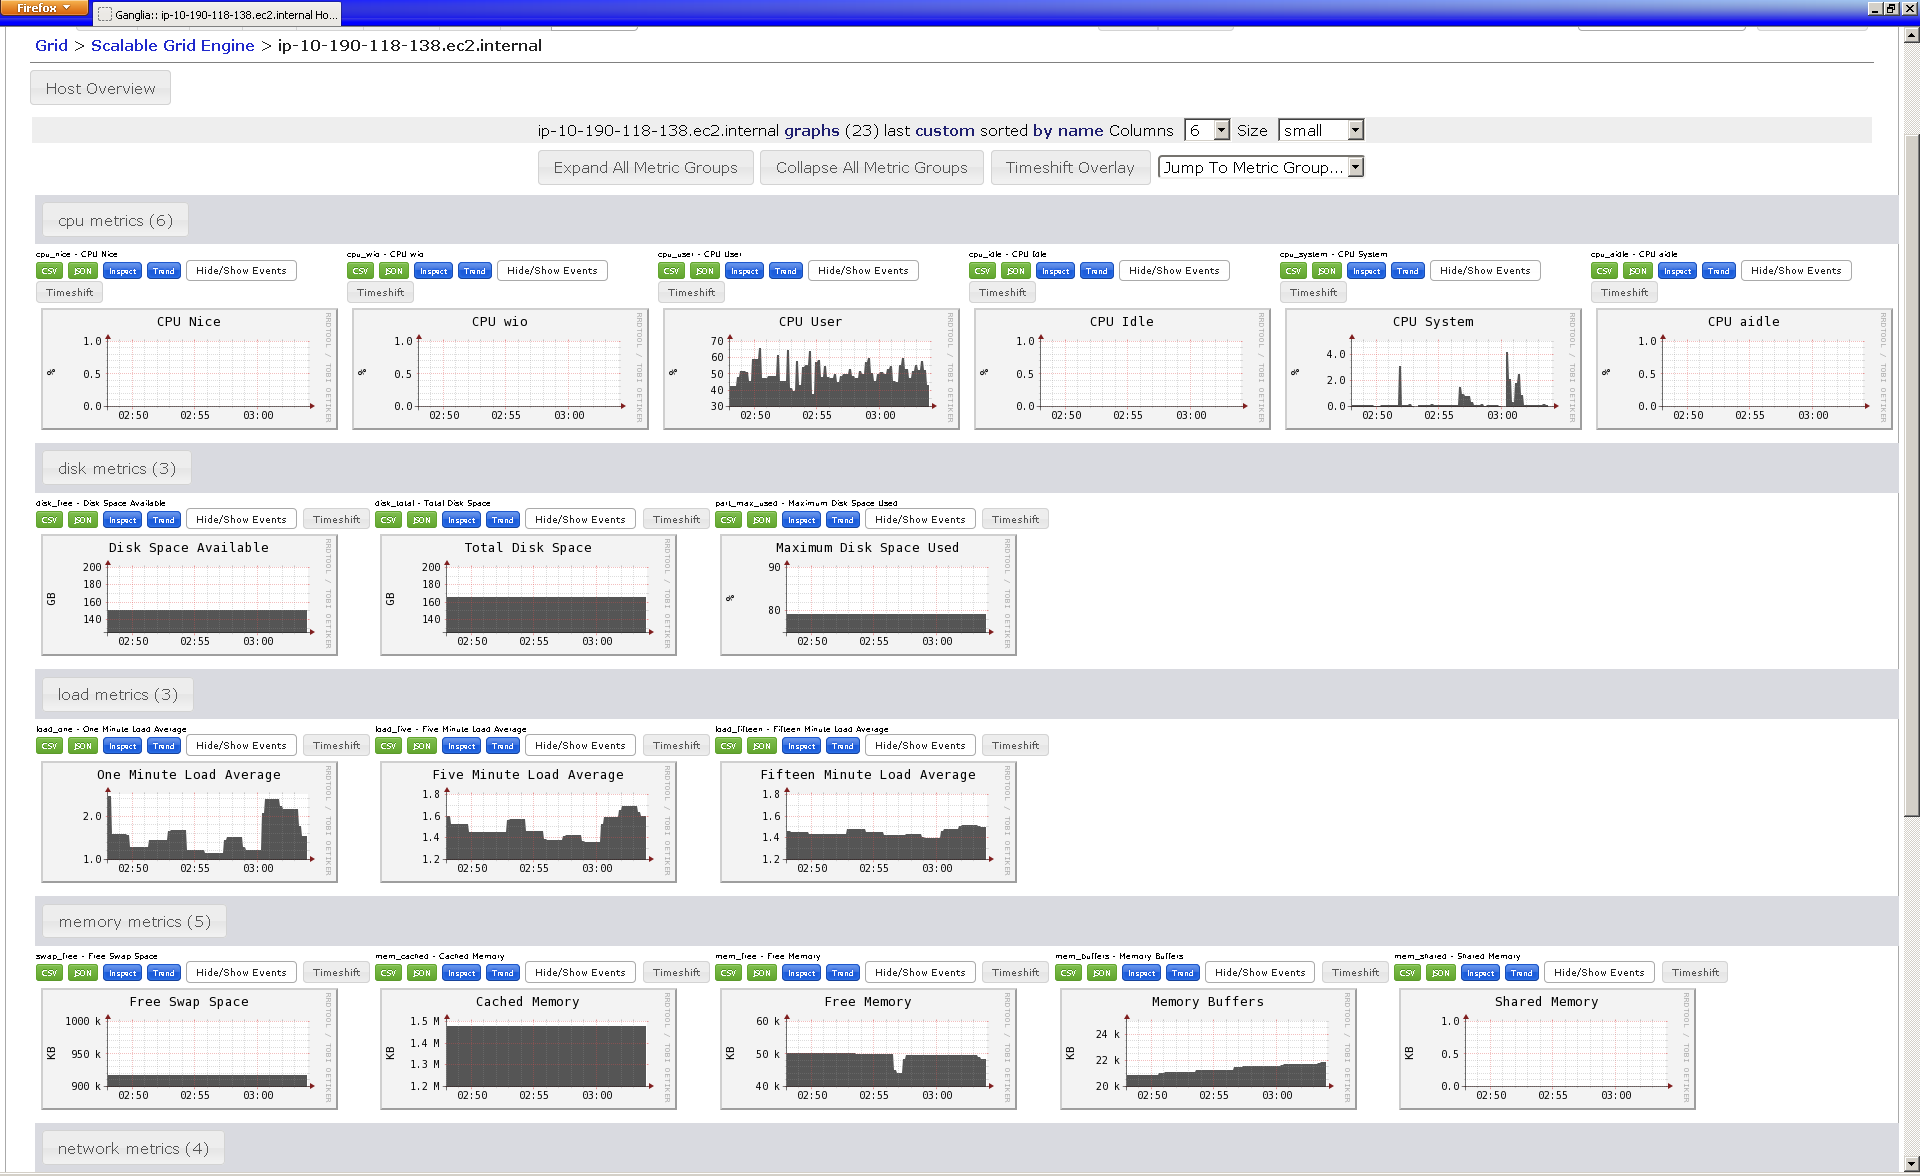
\includegraphics[width=0.9\textwidth]{images/ganglia.png}
    \caption{Screenshot of Ganglia\protect\footnotemark}
    \label{fig:ganglia}
\end{figure*}
\footnotetext{\url{http://en.wikipedia.org/wiki/File:ScalableGridEngineGanglia2.png}}
\begin{figure*}[p]
    \centering
    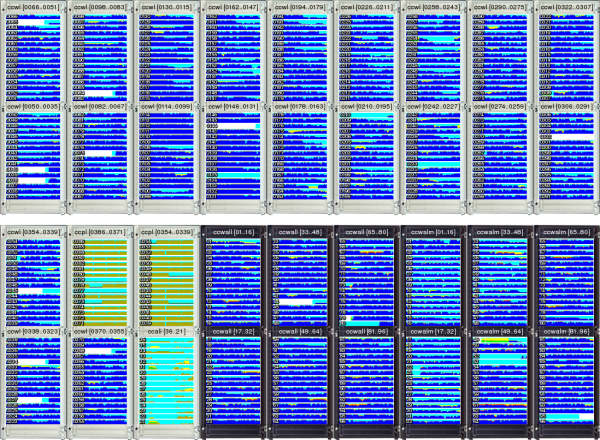
\includegraphics[width=0.9\textwidth]{images/rrdtool.png}
    \caption{Screenshot of RRDtool\protect\footnotemark}
    \label{fig:rrdtool}
\end{figure*}
\footnotetext{\url{http://oss.oetiker.ch/rrdtool/gallery/index.en.html}}

There are many good system monitor solutions out there including Ganglia~\cite{Massie04} and Munin
which is based on RRDtool~\cite{Oetiker99}. However, as you can see in Figure~\ref{fig:ganglia} and
Figure~\ref{fig:rrdtool}, the visualizations become harder to detect anomalies in the system as the
number of nodes increases.

We found Wei Xu and collaborators~\cite{Xu09} made very good system of detecting anomalies by mining
log data. We adopted their machine learning approach including their feature specifications in order
to create an intelligent visualization system.

\section{Methods}
% A detailed explanation of the techniques and algorithms you used to solve the problem.

We have a system which generates such log files using the Google Logging Library
(glog)\footnote{\url{https://code.google.com/p/google-glog/}}. Our goal is to create a generic
visualization library for glog, with emphasis on this system. Theoretically, anybody using glog in a
distributed framework should be able to work with the visualizations out-of-the-box. Here is the
summary of our algorithm:

\paragraph{Algorithm Summary}
\begin{enumerate}
    \item Compute per-node features
        \begin{itemize}
            \item Message count vector
            \item Statistics across time
            \item Each node computes its own features
        \end{itemize}
    \item Select k most representative nodes
        \begin{itemize}
            \item Using distributed k-means clustering
            \item User interactively chooses k
        \end{itemize}
    \item Display interactive visualization
        \begin{itemize}
            \item Client processes visualization
            \item Web server clusters on-demand
            \item Server communicates through Apache server
        \end{itemize}
\end{enumerate}

\subsection{Log Parser}
We mainly used Python for implementing our log parsing system. Google Logging Library provides a
consistent log format so we were able to build a parser easily using Python's regular expression
library. After parsing we need to group every log message by its type and extract nominal and
quantitative data from the messages.

First of all, we group log messages by its source file name and line number. After grouping them
into same types, we could separate dynamic parts of messages from static parts using text difference
algorithms. In Figure~\ref{fig:extracting_data}, you can see an example of extracting data. Since
the dynamic part of log messages will change over time, we can tell the exact part if we have a
large enough amount of log messages of the same type. After detecting dynamic parts, we can simply
parse the part of message strings into integer or floating number if quantitative and string if
nominal.

\subsection{Clusterer}
We also used Python, such as NumPy/SciPy and scikit-learn, for implementing our clustering system.
Due to the huge amount of data we need to preprocess the data in some way to boost the speed of the
clustering up to an interactive rate. As for clustering we used simple k-means clustering
\cite{kmeans,Lloyd82} of the scikit-learn library \cite{scikit-learn} and it turned out the
computation speed is quite good. However, the problem is in the feature extraction. We want to
extract features only from the user-specified time range, i.e., we want to apply clustering on only
features within the range. The range will change continuously by user inputs so we need to be able
to calculate features in real time in order to achieve our goal, an interactive visualization.

We mainly used a message count vector~\cite{Xu09} for our feature vectors and we change the domain
in most cases just by time. Thus, we first came up with data sorted in terms of time. However, just
sorted data structure couldn't help that much because the size of data is still large and it doesn't
fit into the main memory at all. Thus, the data should be stored in a secondary storage, which means
a hard disk drive. Due to the poor performance of random access of hard disk drives we couldn't get
much improvements using the sorted data structure.

Thus, to optimize further we introduced prefix sums of feature vectors. Prefix sums can help
calculating partial sums because we just need to subtract the first element from the last element of
the range to get a sum of values within the range.  We may use Fenwick tree \cite{Fenwick94} or
other advanced data structures but we satisfied with our current performance, which took about 0.4s
per each clustering.

\subsection{Visualization}
\begin{figure*}[p]
    \centering
    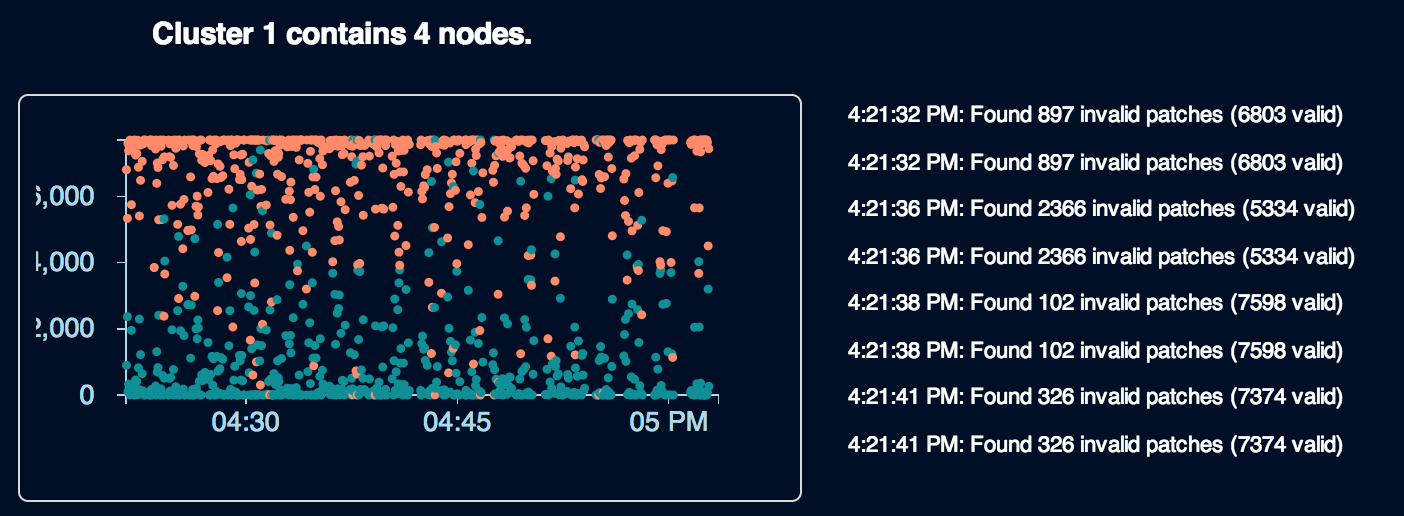
\includegraphics[width=0.9\textwidth]{images/screenshot_plot.png}
    \caption{Data points and raw log messages}
    \label{fig:ss_plot}
\end{figure*}

\begin{figure}[p]
    \centering
    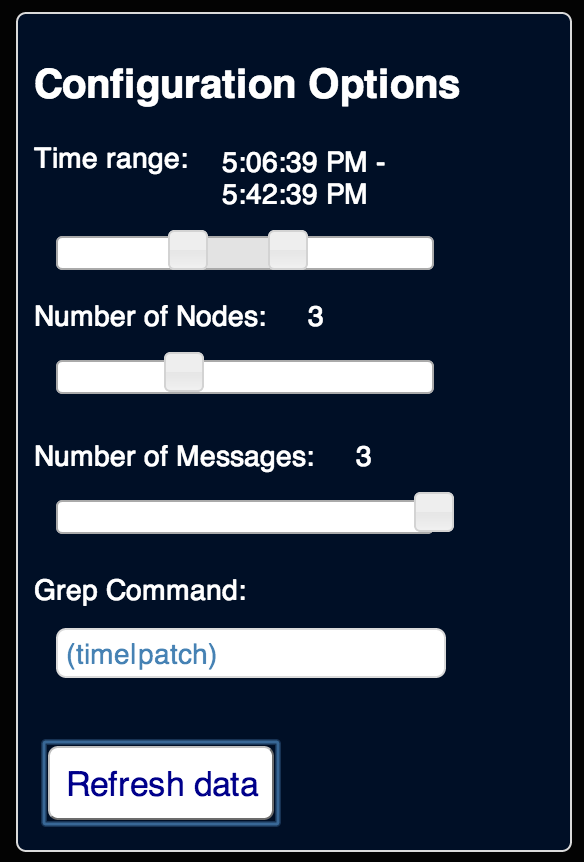
\includegraphics[width=0.7\columnwidth]{images/screenshot_controls.png}
    \caption{User controls}
    \label{fig:ss_controls}
\end{figure}

\begin{figure}[p]
    \centering
    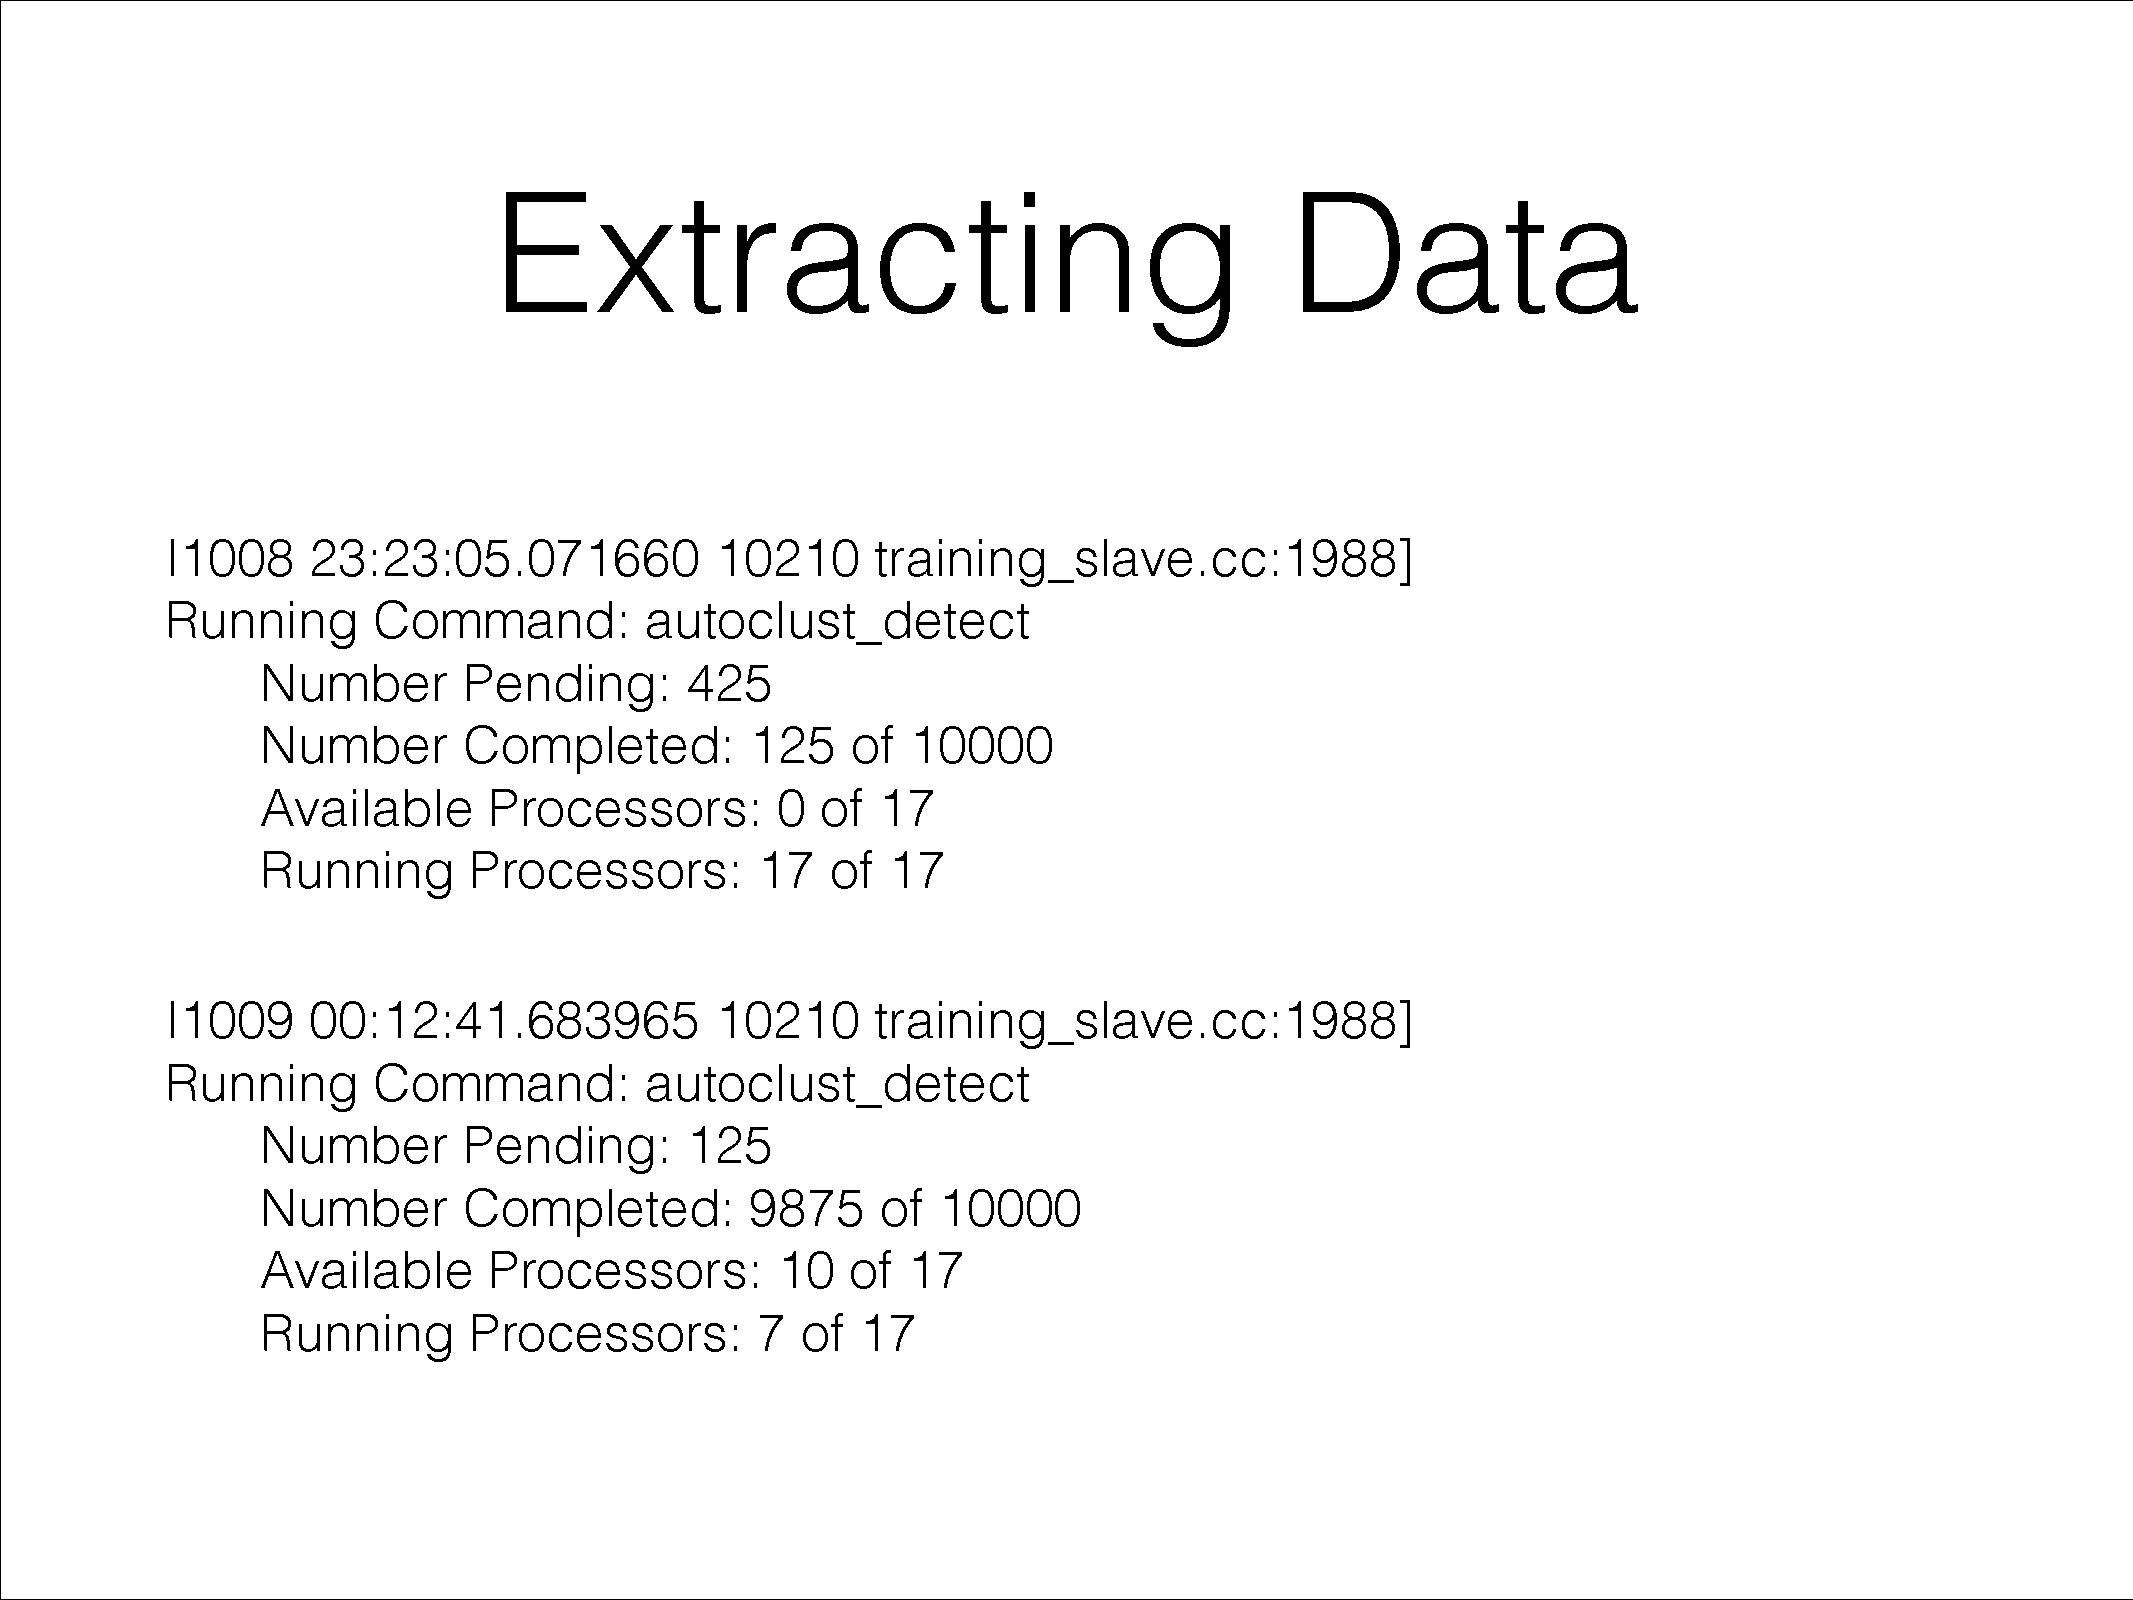
\includegraphics[width=1.0\columnwidth]{images/extracting_data_1.pdf}
    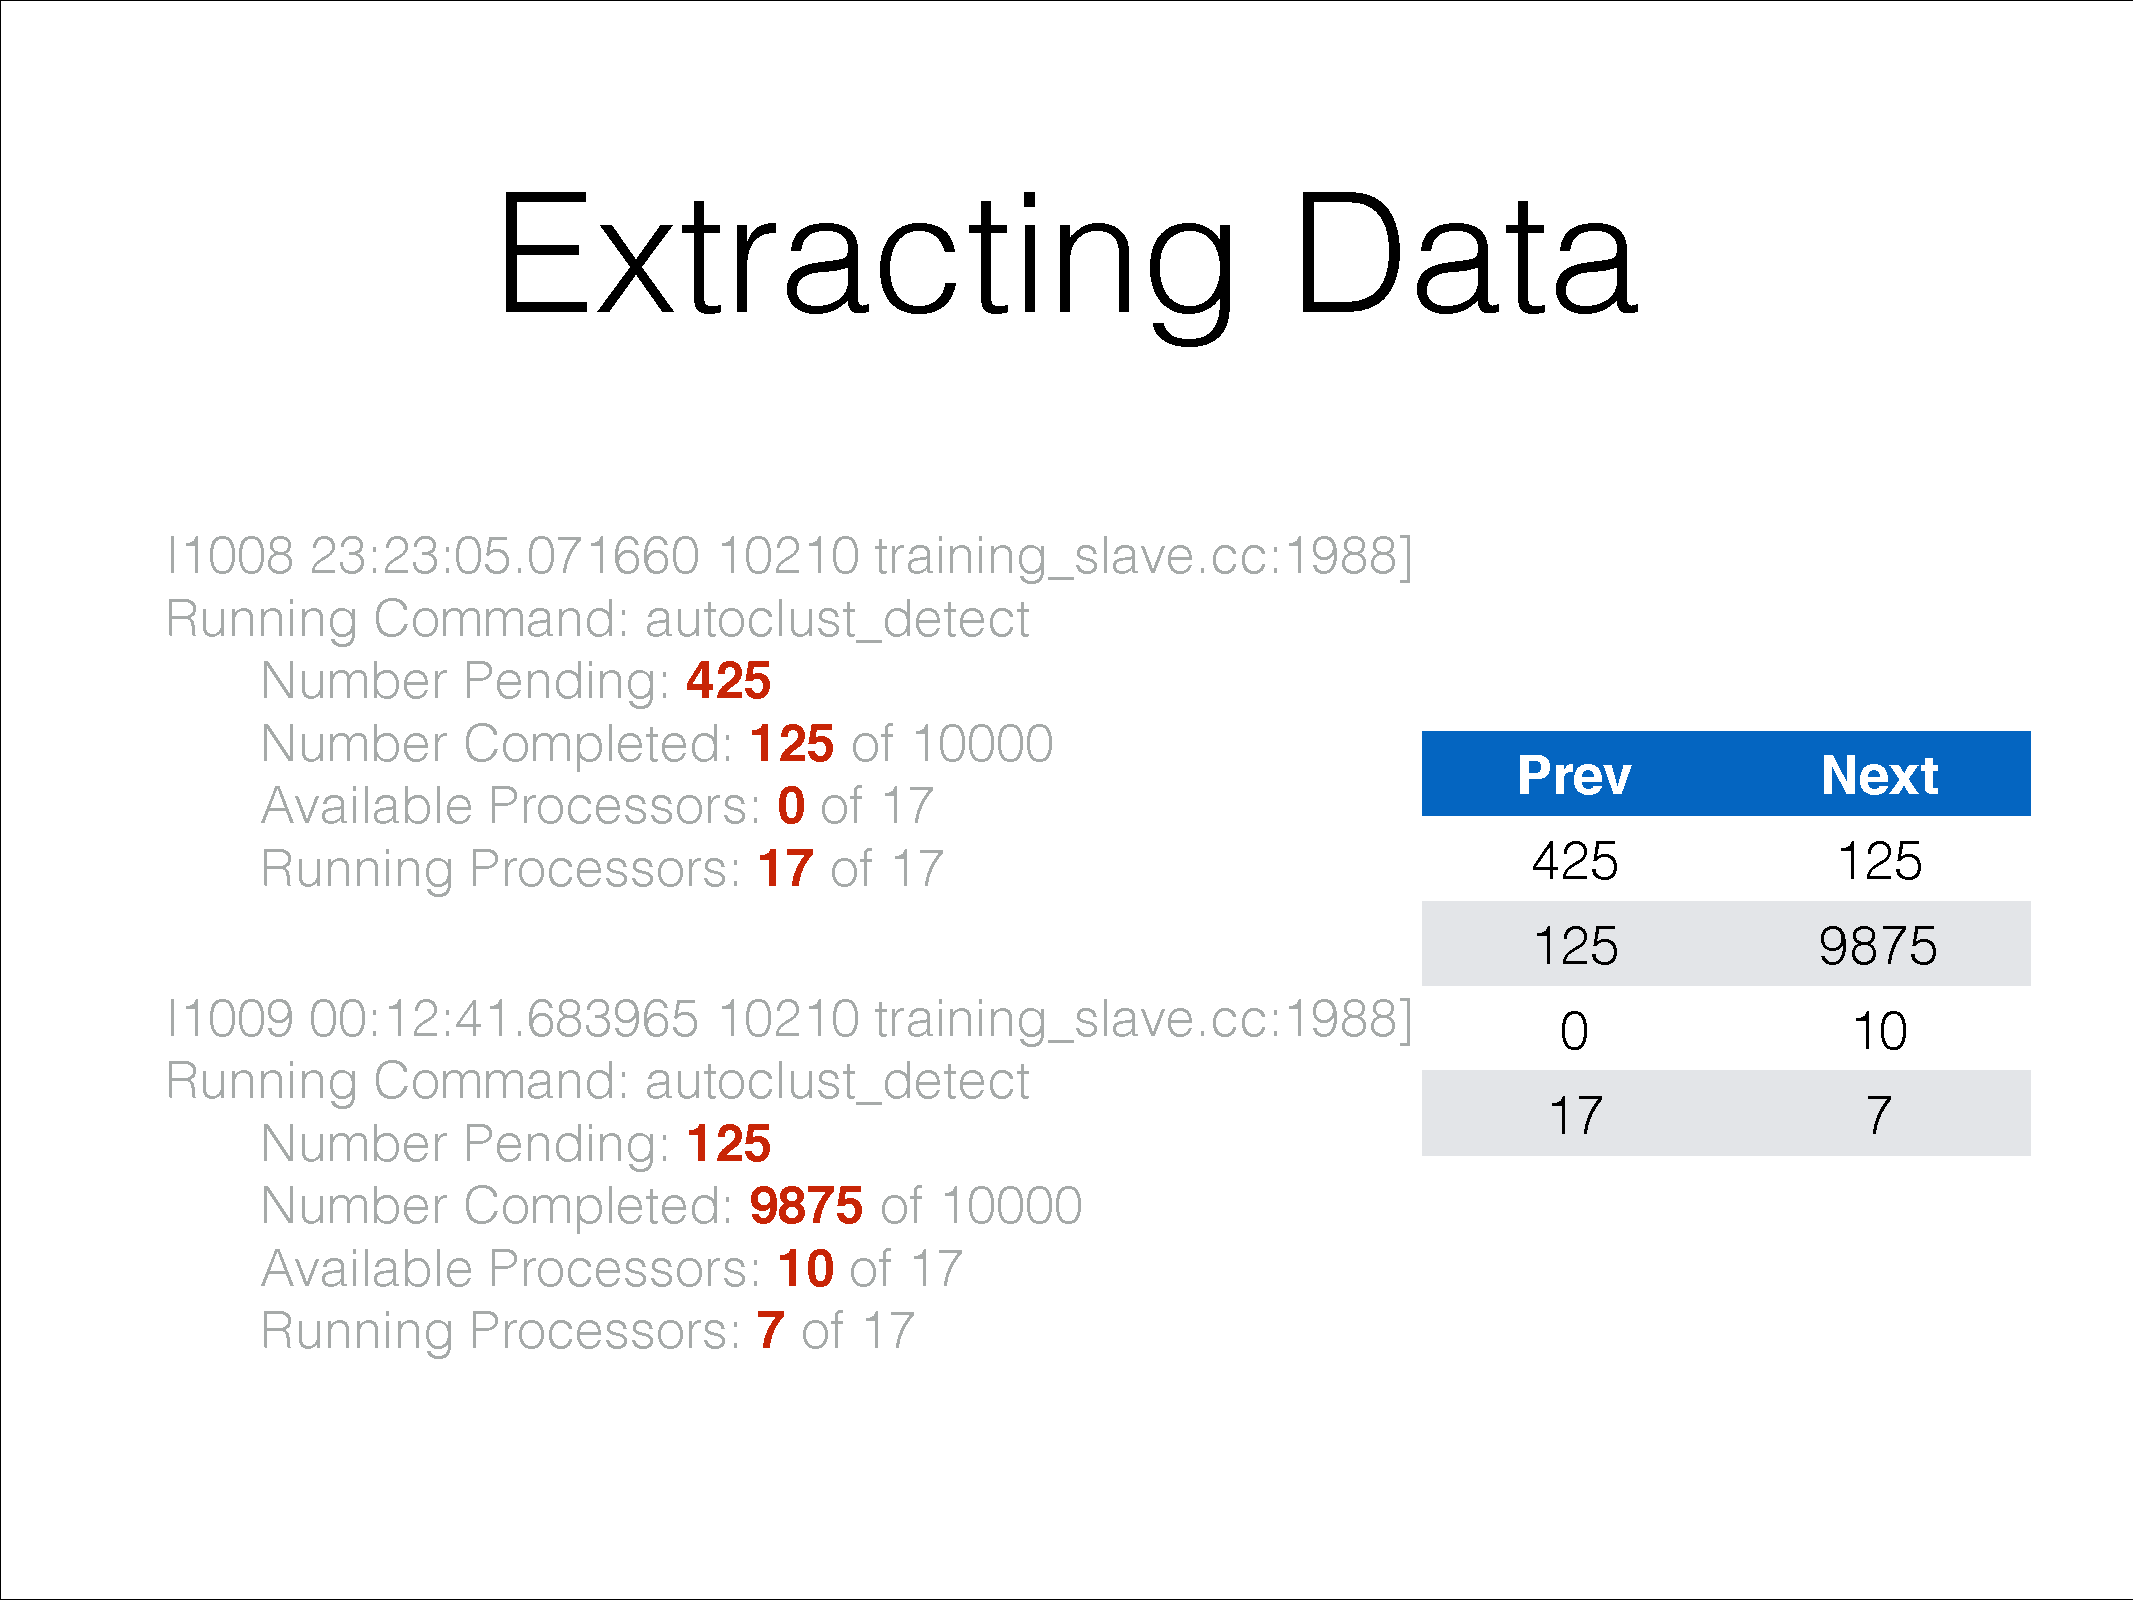
\includegraphics[width=1.0\columnwidth]{images/extracting_data_2.pdf}
    \caption{Text processing}
    \label{fig:extracting_data}
\end{figure}

We used D3~\cite{D311} and jQuery UI libraries for our user interfaces. The front end of our
framework is a web page so that you can explore it using any web browser supporting JavaScript and
SVG. Thus, we can say that we achieved one of our project goals, which is that implementing a system
that easily accessible from remote location using even mobile devices such as a smartphone.

In Figure \ref{fig:ss_controls} you can see the user controls of our visualization. The controls
basically consist of three sliders and one text box and each of them give an user a degree of
freedom in each dimension, such as time, the number of clusters, and the number of message types.

We used one range control for setting time range and two slider control for setting the number of
clusters to find and the number of message types to display, respectively. This system can response
to user inputs at an interactive rate because we speed up the clustering process and now it takes
only a half second as mentioned earlier.

\section{Results}
% The visualizations your system produces and data to help evaluate your approach. For example you
% may include running times, or the time users typically spend generating a visualization using your
% system.

\subsection{Anomaly Detection}
We set the metric for anomaly detection as follow: How many clusters are required until anomalous
node in its own cluster? In the best case of this scenario the number of cluster always should be
two if there is only one type of anomalies at a time.

In Figure~\ref{fig:anomaly} you can see the performance of our anomaly detection and it shows that
our system can tell anomalies such as a failing or slow node under the interference like random
noises. The system works well even when 50\% of the data is garbage, i.e., randomly generated logs.

\begin{figure}[p]
    \centering
    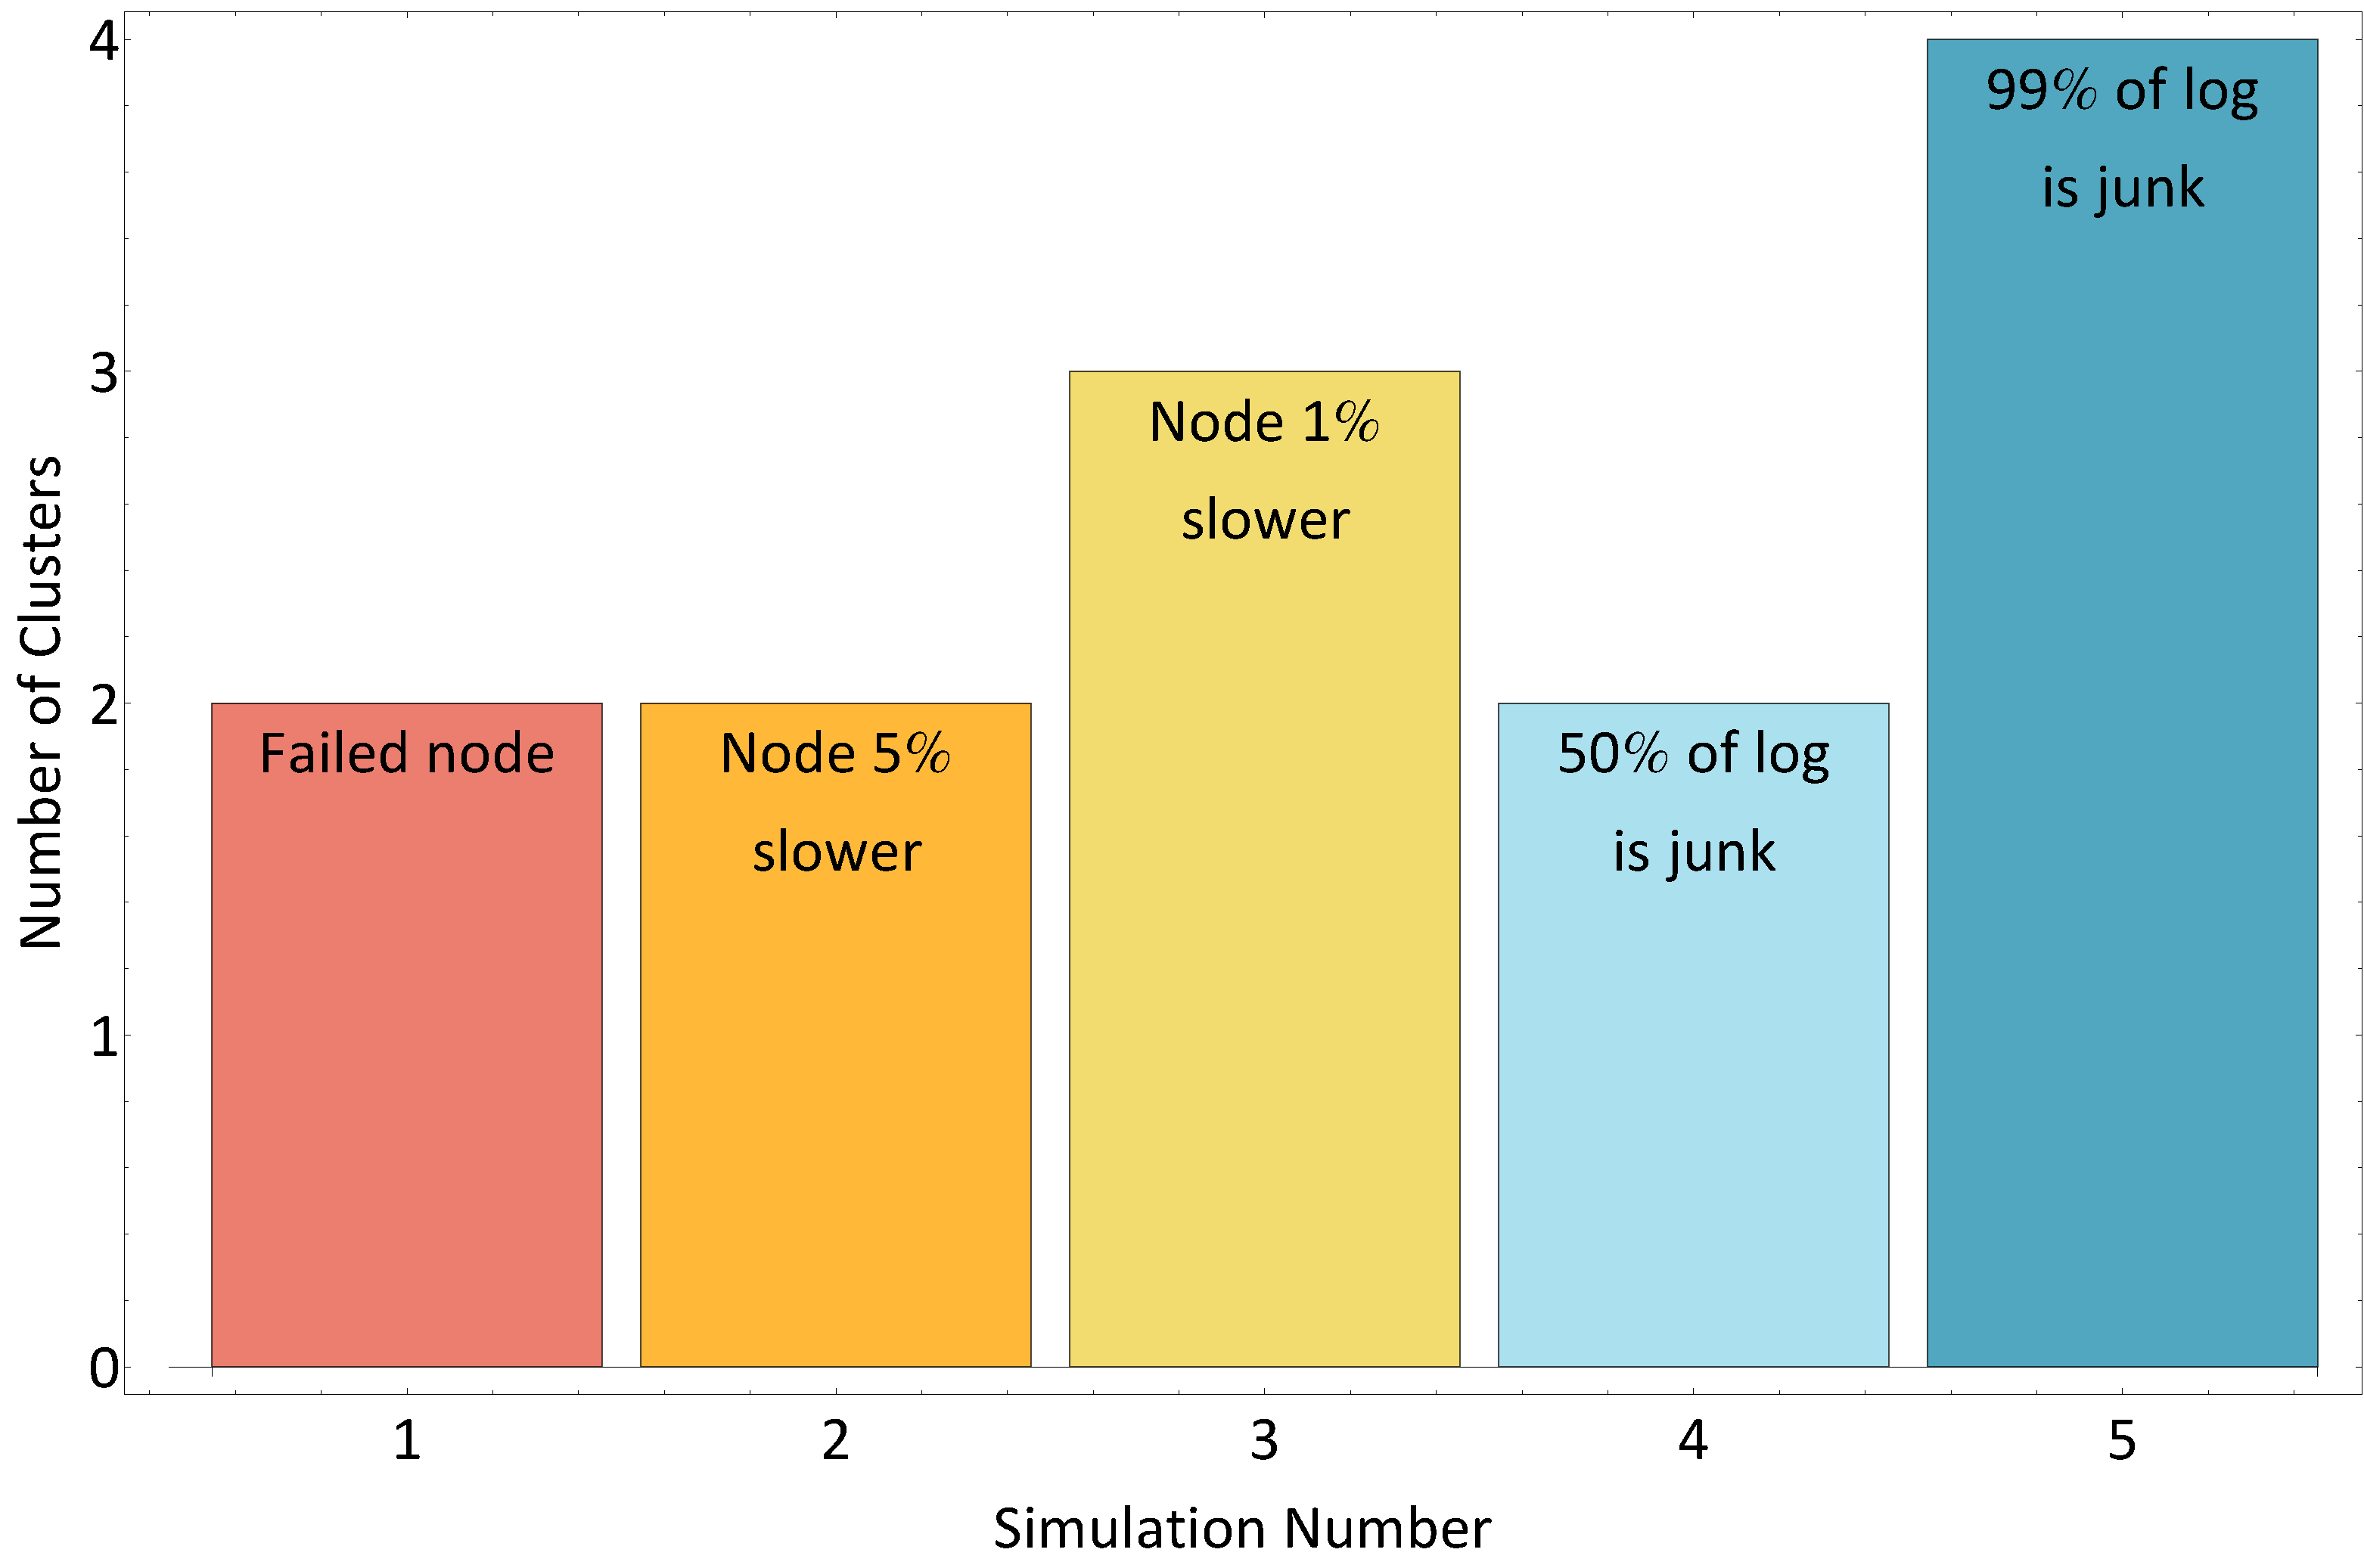
\includegraphics[width=1.0\columnwidth]{images/anomaly.pdf}
    \caption{Anomaly detection}
    \label{fig:anomaly}
\end{figure}

If we were able to find a ground-truth log file with labeled anomalies, we could compare our error
rates to those presented in papers by Wei Xu et al. Unfortunately, we couldn't find any publicly
accessible log database.

\subsection{Timing Information}
We ran on 500,000 messages per node and on average 30MB of data were sent to the HTTP Server per
node. Visualization took on the client side so the computation cost of visualization doesn't slow
down the server. In Figure~\ref{fig:timings} you can see basic timing information of our system.

\begin{figure}[p]
    \centering
    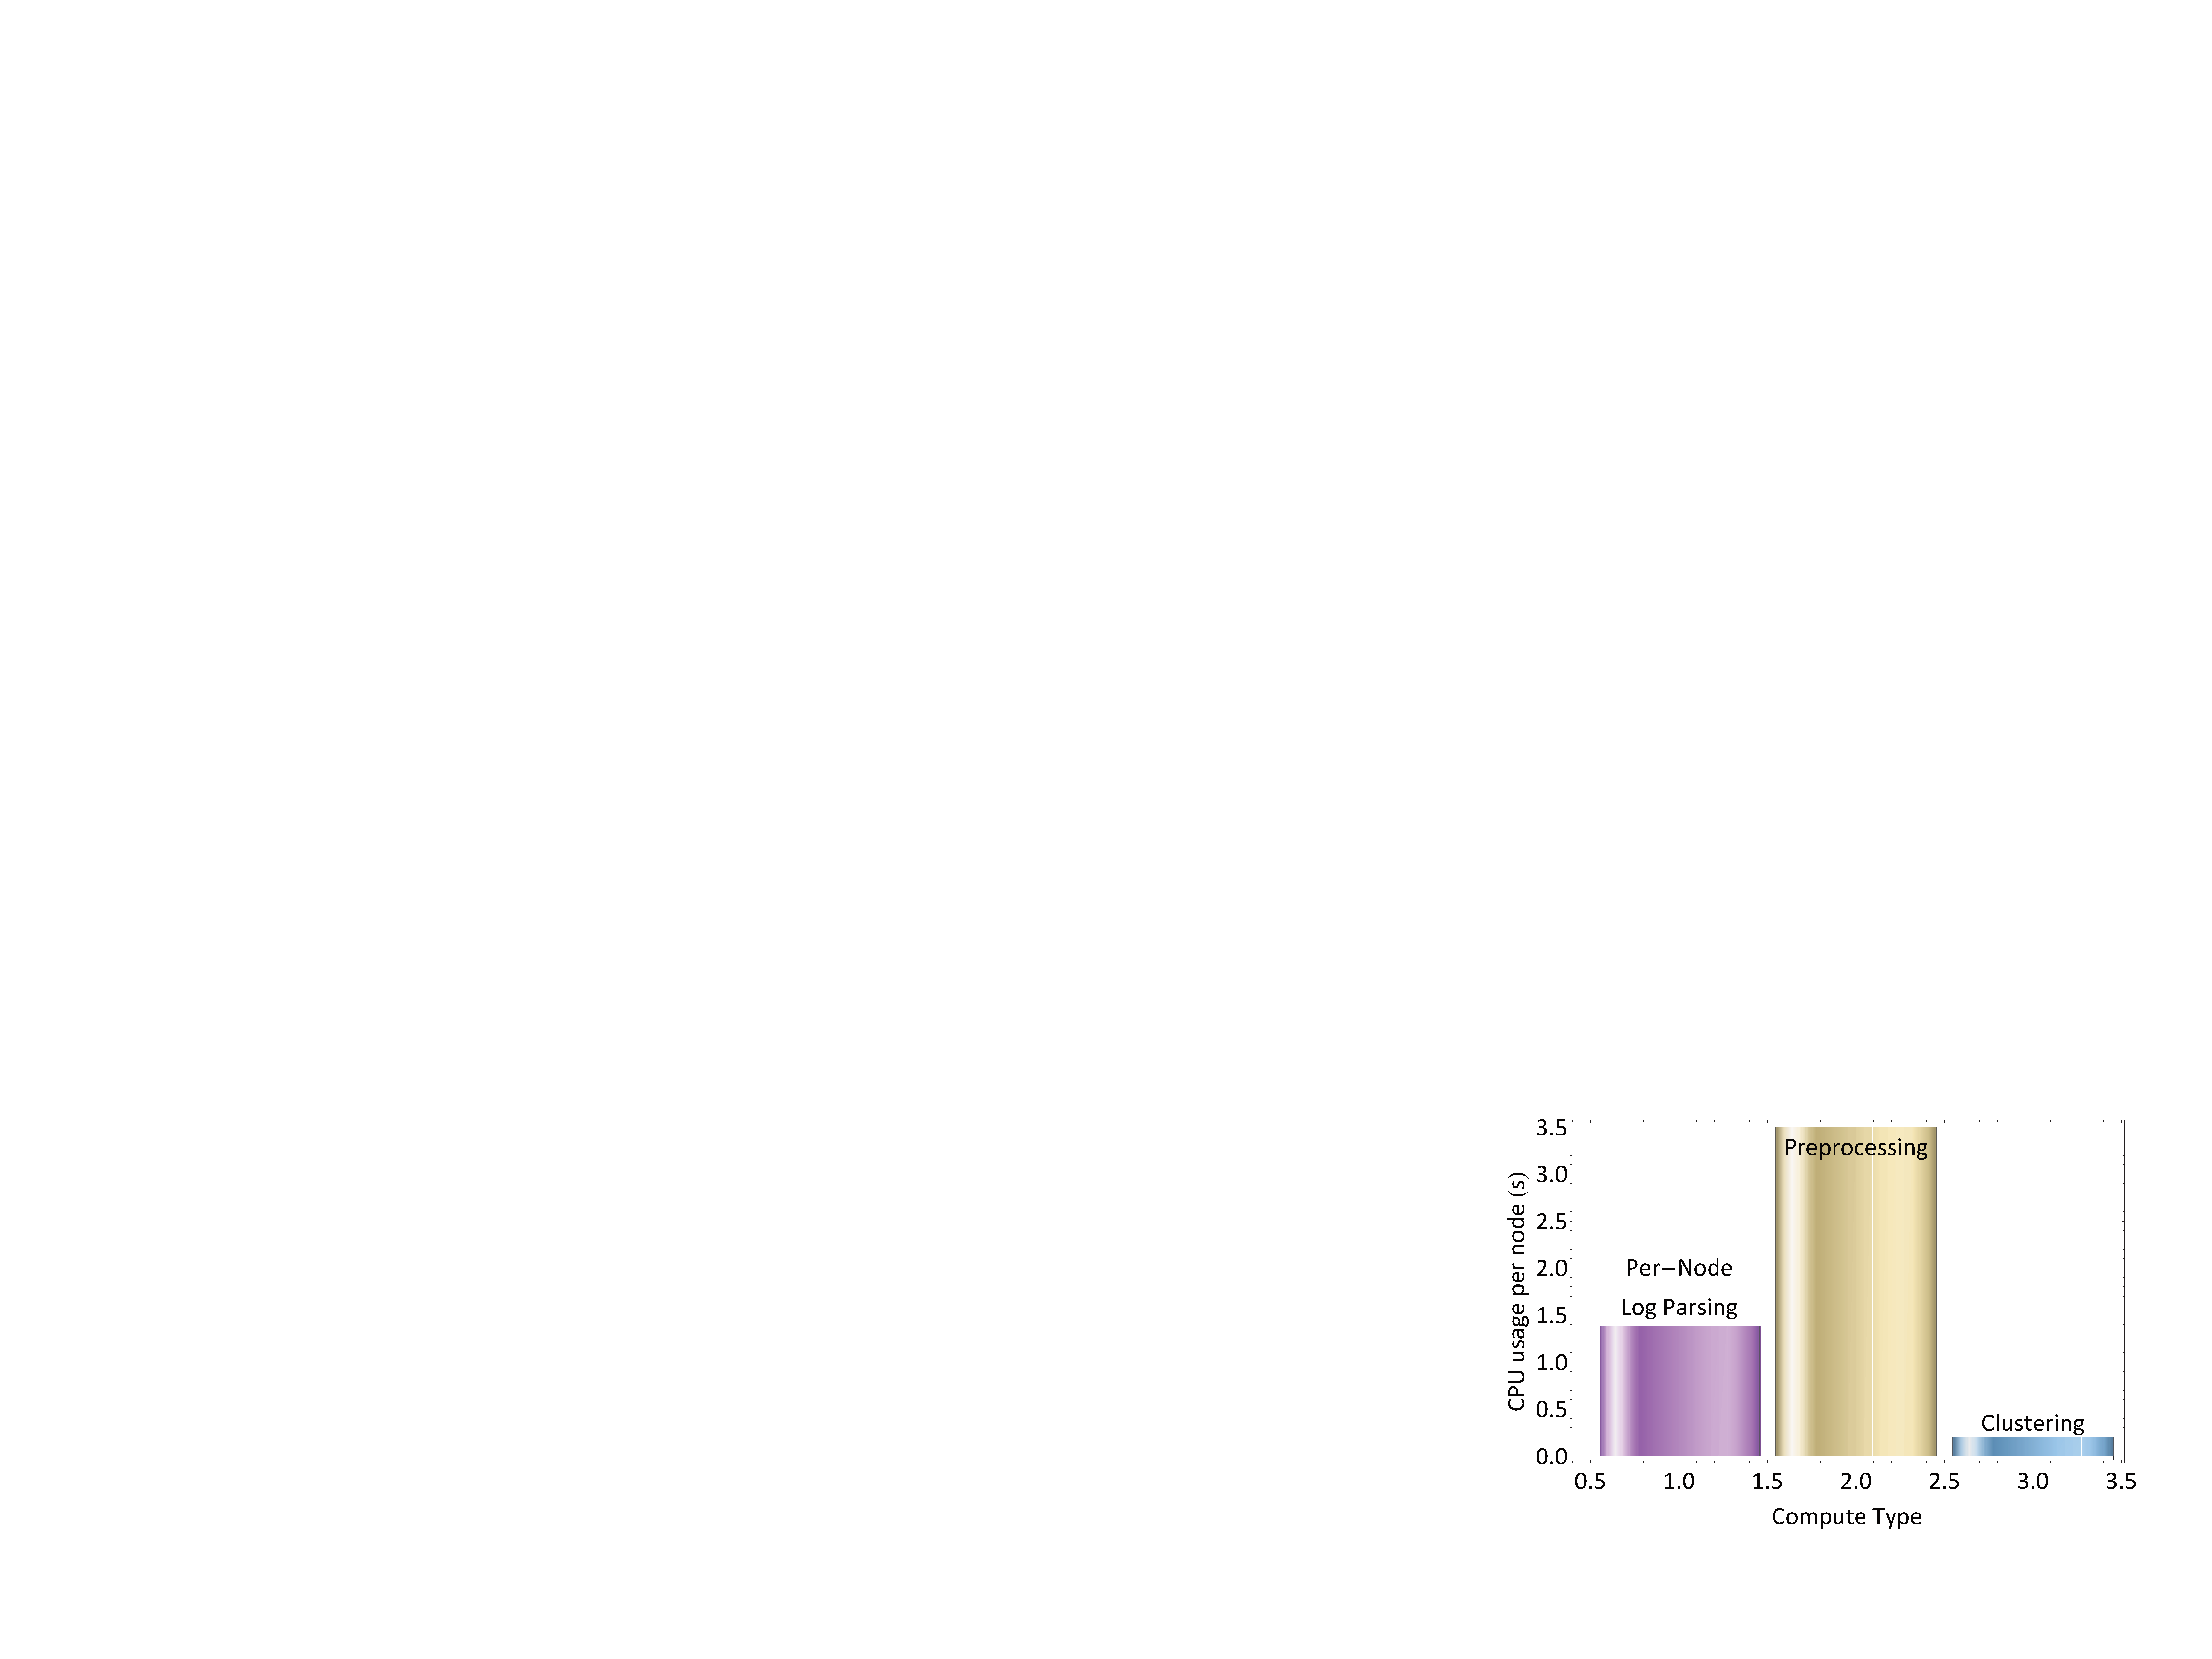
\includegraphics[width=1.0\columnwidth]{images/timing.pdf}
    \caption{Timing information}
    \label{fig:timings}
\end{figure}


\section{Discussion}
% What has the audience learned about visualization from your work?

The log data we used in this project came from the system which looks through terabytes of Google
Street View data and uses them for various machine learning tasks. It uses about 80 processes, each
process with its own log file, and spread over around a dozen machines. There are regular failures
which are currently cumbersome to find and debug.

We wanted to create a responsive system which visualizes the state of the system in real-time, is
robust to errors, and can display an arbitrary number of nodes. Not all nodes will be displayable on
a single screen, so the system had to be able to determine areas of interest (e.g. failed nodes,
slow nodes, or completed tasks) in the visualization and direct the user’s attention there. Our
anomaly detection built on Wei Xu's in several ways: (1) their work does not use timestamps, which
we believe are vital to understanding the system’s state; (2) their work intentionally ignores the
ordering of log messages, and instead pays attention only to the number of occurrences of a message
, we hypothesize order may matter; (3) most importantly, their visualizations are more primitive. We
believe the idea of near-infinite zoom (where the most detailed layer essentially shows the
information in the actual log, and as you zoom out, more and more information is aggregated) will
allow a user to explore the system state rapidly.

What we want to point out in this paper is that along with our project there is a direction of
visualization research that can ultimately help system administrators to monitor and analyze the
status of a large distributed system. We think this will become more and more important as the trend
of technology emphasizes on parallelism and distributed system such as cloud computing.


\section{Future Work}
% A description of how your system could be extended.}

We believe automatically determining plot type would be a good improvement for our system because
data extracted from raw log messages can be arbitrary and it is hard to be predetermined by an user.
Also, we want to extend our system to online and real-time analysis and implement more intelligent
features preprocessing. Lastly, it would be great if our system can cluster logs based on more
elaborate features.

\section*{Acknowledgements}
The authors appreciate Ling Huang for his helpful advices and Sean Arietta for providing the log
data gathered from his research project.


\bibliographystyle{style/acmsiggraph}
\bibliography{paper}
\end{document}
